\documentclass[11pt]{article}
\usepackage{amsmath, geometry, enumerate, algorithm2e}
\usepackage{graphicx}
\usepackage[toc,page]{appendix}
\geometry{margin=1.5in}
\setlength{\textheight}{8.75in} \setlength{\topmargin}{-.2in}
\setlength{\headheight}{.2in} \setlength{\headsep}{0in}

\begin{document}
\begin{titlepage}
	\begin{center}
		\vspace*{1in}	
		\Huge
		\textbf{Verification of $\alpha$-Approximately-Sorted Lists}
		\vspace{.5in}
		
		\Large
		\text{Randomized Algorithms Final} \\
		\text{Spring 2016}
		
		\vspace{1.5in}
		
		\textbf{Chris Celi \\ Mark Westerhoff}
	\end{center}
\end{titlepage}

\clearpage

\tableofcontents

\clearpage

\section{Introduction}

In this paper we present an algorithm that verifies a (potentially large) list of integers is $\alpha$-approximately-sorted ($\alpha$AS). As no clear definition to what precisely `sorted' means, we present one as well. 

A list $L = \{a_1, a_2, ..., a_n\}$ is perfectly sorted if for all $i \in [2, n]$, $a_{i-1} \leq a_i$. Consequently a list of size 1 is always sorted so the case where $i = 1$ is ignored. Intuitively this boils down to if each element must be increased to reach the next element (including an increase of zero) then the list is perfectly sorted. 

A more interesting case however is when a list is $\alpha$AS. A list $L = \{b_1, b_2, ..., b_n\}$ is $\alpha$AS sorted for some $\alpha$ such that $0 \leq \alpha \leq 1$, if for all $i \in [2, n]$, $\Pr[b_{i-1} \leq b_i] \geq \alpha$. Thus a perfectly sorted list is also $\alpha$AS when $\alpha = 1$. Providing some more intuition, the probability that each element is greater than or equal to element prior is lower bounded by $\alpha$. We operate with this assumption as a definition for the design of the algorithm. 

\subsection{Problem Analysis}

Simply verifying if a list is $\alpha$AS is infeasible to do linearly (in accordance with the definition provided) when the list is on the scale of several billion elements. Instead we take a randomized approach to the problem in order to break down the task at hand. 

Suppose we are provided a list $L = \{a_1, a_2, ..., a_n\}$ where $n \geq 10^9$, and some $\alpha$ where $0 \leq \alpha \leq 1$. Then we define a collection of $n-1$ variables $X_1, ..., X_{n-1}$ to be a metric for if each sequential pair of terms in the list is sorted. Thus we define $X_i$ as
$$X_i = 
\begin{cases}
	1 & a_{i-1} \leq a_i \\
	0 & \text{ otherwise}
\end{cases}$$
and as a result if we let $X = \sum X_i$, then $X$ is a metric for the sorted nature of the entire list. This presents an easy way to verify if a list is $\alpha$AS by having the algorithm return true when $E[X] \geq \lceil \alpha n \rceil$ and false when $E[X] < \lceil \alpha n \rceil$.

Instead of checking each term linearly, we can approximate $E[X]$ using randomized means. 

\section{Algorithm}

We can approximate $E[X]$ using a Monte Carlo method. We sample from $X$ various values $X_i$ which are all easily computed in sub-linear time based on $L$. This is done by pulling out only the two necessary numbers for each $X_i$ selected and seeing which case $0$ or $1$ applies. Naturally we are able to sample from $X$ uniformly and at random and do not need to generate the full list to determine any $X_i$. Using a Monte Carlo method, and a sample of size $k$, we know that $E[X] = n \sum\limits^k_{i=1} \frac{X_i}{k}$ from Motwani and Raghavan \cite{textbook}. We devise an algorithm to approximate $E[X]$ as $\alpha$-estimate and compare that value to the provided $\alpha$. 

\subsection{Assumptions}

A few of assumptions are required concerning the input in order to be allowed some of the theoretical assurances discussed in this paper. They are as follows:

\begin{enumerate}

\item The input must be provided as a file where each number is padded (with zeros perhaps) to ensure that each number is the same length. This allows us to use offsets when seeking the file to jump quickly and accurately to specific values of $a_i$. In other words, access to $a_i$ is desired to be constant time (i.e. a quick offset calculation and jump to location in a file). This is a very strict requirement that directly affects the runtime of the algorithm. 

\item The input file must be large. The Monte Carlo method works best on larger input sizes, and so we require that $n \geq 10^9$. In practice, we generate a $k$ sample size which is independent from $n$. Thus $n$ must be sufficiently large for the algorithm to make sense at all.

\item The desired value for $\alpha$ is known and is relatively close to $1$. Later we will derive a sample size based on $\alpha$ which scales best with larger sizes of $\alpha$. For this algorithm and testing we say that we are looking for an $\alpha \approx .9$. We have not tested the algorithm when $\alpha$ was significantly lower. It is very important that the lists tested be relatively close to $\alpha$ sorted as the theory depends on it. 

\end{enumerate}

\subsection{Specification}

The algorithm is as follows. It is important to note that it is an $(\epsilon, \delta)$-fully polynomial-time randomized approximation scheme ($(\epsilon, \delta)$-FPRAS) like other Monte Carlo algorithms. 

\vspace{.15in}

\begin{algorithm}[H]
	\KwData{A file of $n$ integers to be verified, $\alpha$, $\epsilon$, and $\delta$.}
	\KwResult{True if the list is $\alpha$AS, false otherwise.}
 
 	load file\;
 	$k = \frac{4}{\epsilon^2 \alpha} \ln \frac{2}{\delta}$\;
	$sum = 0$\; 
 
 	\For{i from 1 to $k$}{
 	
 		$x = \text{random index of a value pair with replacement}$\;
 		$v_1, v_2 = \text{get sequential value pair for } x$\;
 		
 		\If{$v_1 \leq v_2$}{
 			$sum++$\;
 		}
 	}
 	
 	$\alpha$-estimate = sum $\div$ $k$\;
 	\Return ($\alpha$-estimate $\geq \alpha$)\;
 	\vspace{.15in}
 	\caption{A Monte Carlo-based verification algorithm for $\alpha$AS lists.}
\end{algorithm}

\subsection{Runtime Analysis}

As we mentioned, with the given assumptions, loading the file and retrieving each pair from the file is considered $O(1)$. Thus the algorithm is trivially $O(k)$ and scales with the size of the sample set used. 

\section{Theoretical Analysis}

Remember that the random variables $X_i$ have the Bernoulli distribution with parameter approximately $\alpha$. We will say that the true parameter is $\beta$. That is, the lowest value of $\alpha$ that would return true for the given list would be $\beta$. 

Using the Estimator Theorem from Motwani and Raghavan \cite{textbook}, with $\beta$ being the ratio of sorted elements to total elements, the Monte Carlo method yields an $\epsilon$-approximation to the number of sorted elements with probability at least $1-\delta$ given a sample size of size $$k \geq \frac{4}{\epsilon^2 \beta} \ln \frac{2}{\delta}.$$ 

The result of this theorem is a bound on $E[X]$ as $$\Pr\left[ [(1-\epsilon)\beta n] \leq E[X] \leq [(1+\epsilon)\beta n] \right] \leq 1 - \delta.$$ where $\beta n$ refers to the true number of sorted pairs. 

We can simplify this further by removing the factor of $n$ from each term to yield $$\Pr\left[ [(1-\epsilon)\beta] \leq \alpha \leq [(1+\epsilon)\beta] \right] \leq 1 - \delta.$$

Thus we have a method of estimating the true approximately sorted value of the given list. However, our sample size depends on an unknown value $\beta$. From our third assumption we approximate $\beta$ with $\alpha$ which is known from the specification of the algorithm. A lower $\alpha$ value will lead to a drastically increased value for $k$ increasing the corresponding runtime. This can be seen in Figure 1.

This leaves us with $$k \geq \frac{4}{\epsilon^2 \alpha} \ln \frac{2}{\delta}$$ where we commonly use $\alpha = .9$ for testing the algorithm. It is rather important to note that $k$ is not dependent on $n$ in any way. Thus this algorithm scales well, especially on larger inputs.

The algorithm produces two-sided error however. Going back to our probabilistic bounds, the probability that the algorithm yields an $\alpha$-estimate that is within $\epsilon$ of $\beta$ is $1 - \delta$. We can then compare the produced $\alpha$-estimate to the verification metric ($\alpha$) provided from the onset. 

The algorithm though, needs to verify whether or not a list is $\alpha$AS. This can be done by requiring a small $\epsilon$ to tighten the window for our $\alpha$-estimate. The $\alpha$-estimate can also be tightened by boosting the algorithm with multiple iterations. By running the algorithm $i$ times, we see that the probability that $\alpha$-estimate is within $\epsilon$ of $\beta$ is $1 - \delta^i$. Depending on the relaxation of runtime, the result can be boosted to the desired constant. Even with large $\delta$ values, (such as $\delta = .25$) the rate at which $1 - \delta^i$ converges to $1$ is very fast. Thus not many iterations are required; these results can be seen in Figure 2. This leads to a very confident result rather quickly.

\section{Experimental Analysis}

We developed Python code to do some simple testing of our algorithm. The code repository can be found here: \textbf{https://github.com/celic/alpha-sort}. To begin testing, we generated four different datasets of one billion numbers with $\beta \approx 0.9$. Warning: Given that we pad each number for easier seeking, generating each file to approximately 90 minutes and took up 11GB. 

First, we tested the consistency of the program. We ran 1000 simulations with $\epsilon=0.1, \delta=0.25, \alpha=\beta$, and with only one iteration. We expect 75\% of the simulations to result with $\alpha$-estimates within the error bound. The largest error noticed was $0.039$, which is well within $\epsilon$. We repeated this with several other sets of values, and the results always seemed to be within the bounds. We are unsure as to why this occurred exactly.

Performance wise, the code executed very quickly. For any practical set of values, using just one iteration (i.e. no boosting), computing the algorithm ran in just a fraction of a second. Worst case, with 16 iterations, it still only took a few seconds. On top of this, on average over 95\% of execution time was spent doing I/O. This makes sense as I/O is much slower, and $2k$ numbers need to be read, whereas only $k$ calculations are performed (and are much faster). However, if this algorithm was put into production, it would be trivial to parallelize the I/O, providing significant performance boosts to our already very fast algorithm. Overall, we did not perform extensive testing, but from the results so far, our approach seems very promising.

\section{Conclusion}

This algorithm performs surprisingly well for how simple it is in design. By pulling $k$ samples from the $n$ sized list and predicting the $\beta$ value for the list we end up with a very accurate verification algorithm based on $\alpha$. It is important to note that the size of $k$ does not scale with $n$ which is a very pleasing result. This allows the size of the list to potentially be unlimited in size.  

\newpage
\addcontentsline{toc}{section}{Appendix}
\begin{appendices}

\begin{figure}[h!]
	\centering
	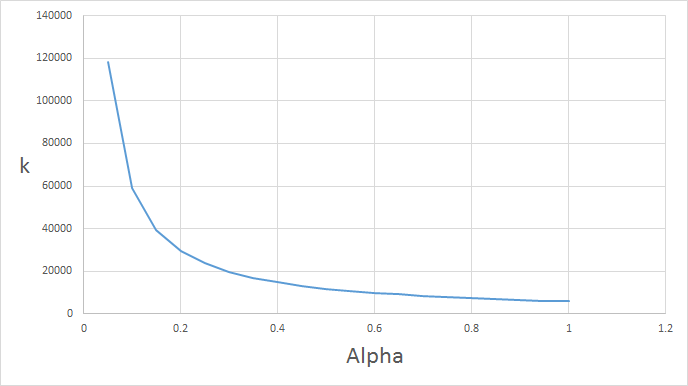
\includegraphics[width=0.7\linewidth]{fig1.png}
	\caption{How the sample size (k) is affected by the value of $\alpha$.		
		This shows that the sample size grows exponentially as $\alpha$ decreases. This one of the reasons for assumption three.
		Note: $\epsilon=0.05$ and $\delta=0.05$.}
\end{figure}

\begin{figure}[h!]
	\centering
	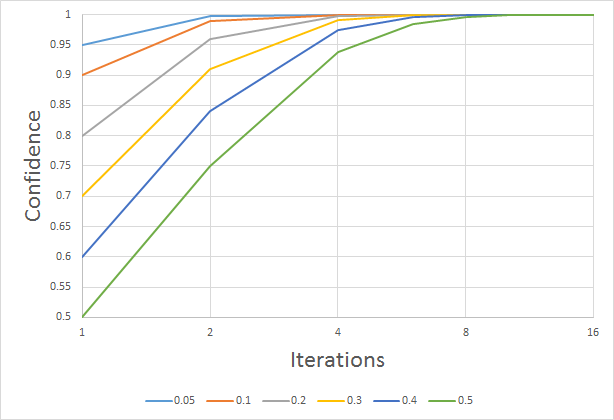
\includegraphics[width=0.7\linewidth]{fig2.png}
	\caption{The confidence that the $\alpha$-estimate is within the error bound $\epsilon$ by the number of iterations. Each line represents a different $\delta$ value. This Figure demonstrates how even with very large (and impractical) values of $\delta$, it still takes a very small amount of iterations to have nearly full confidence that the result is within the $\epsilon$ bound.}
\end{figure}
\end{appendices}

\newpage
\addcontentsline{toc}{section}{References}
\begin{thebibliography}{2}

\bibitem{textbook}
Rajeev Motwani, and Prabhakar Raghavan.
\textit{Randomized Algorithms}. 1995. 9th ed.
Cambridge University Press, 2007.
311-313. Print.

\end{thebibliography}

\end{document}
